\documentclass{beamer}

\setbeamertemplate{caption}[numbered]
\usetheme{Hannover}
\usepackage{subcaption}
\expandafter\ifstrequal\expandafter{\jobname}{notes}{
  \setbeameroption{show only notes}
}{
}

\begin{document}

% TODO: make Oxford template

\title{Firefly: Exploiting Implicit Trust in Satellite Downlink Processing Systems}
\author[Edd Salkield]{
  \emph{Edd Salkield}
  \inst{1}
  \and
  Joshua Smailes
  \inst{1}
  \and
  Richard Baker
  \inst{1}
  \and
  Martin Strohmeier
  \inst{2}
  \and
  Ivan Martinovic
  \inst{1}
}
\institute[University of Oxford]{
  \inst{1} Systems Security Lab, University of Oxford \and %
  \inst{2} Cyber-Defence Campus, armasuisse Science + Technology
}
\date{Trinity Term 2022}

\begin{frame}
  \titlepage
\end{frame}

\section{Motivation}

\begin{frame}
  \frametitle{What's new in space?}
  \framesubtitle{Large constellations, satellite miniaturisation}
  \begin{columns}[t]
    \begin{column}{5cm}
      \centering
      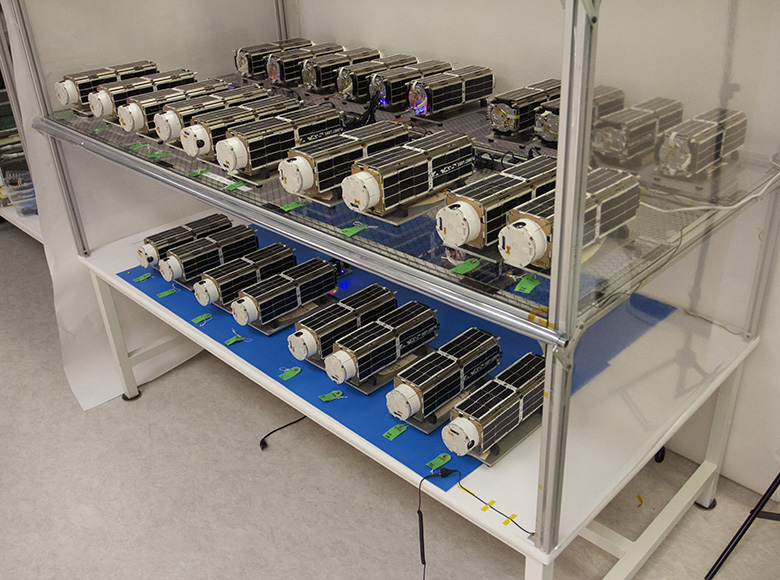
\includegraphics[width=\columnwidth]{images/planetlabs_satellites.jpg}
      \newline
      Planet labs dove satellites~\footnote[frame]{Image: Planet Labs}
    \end{column}

    \begin{column}{5cm}
      \centering
      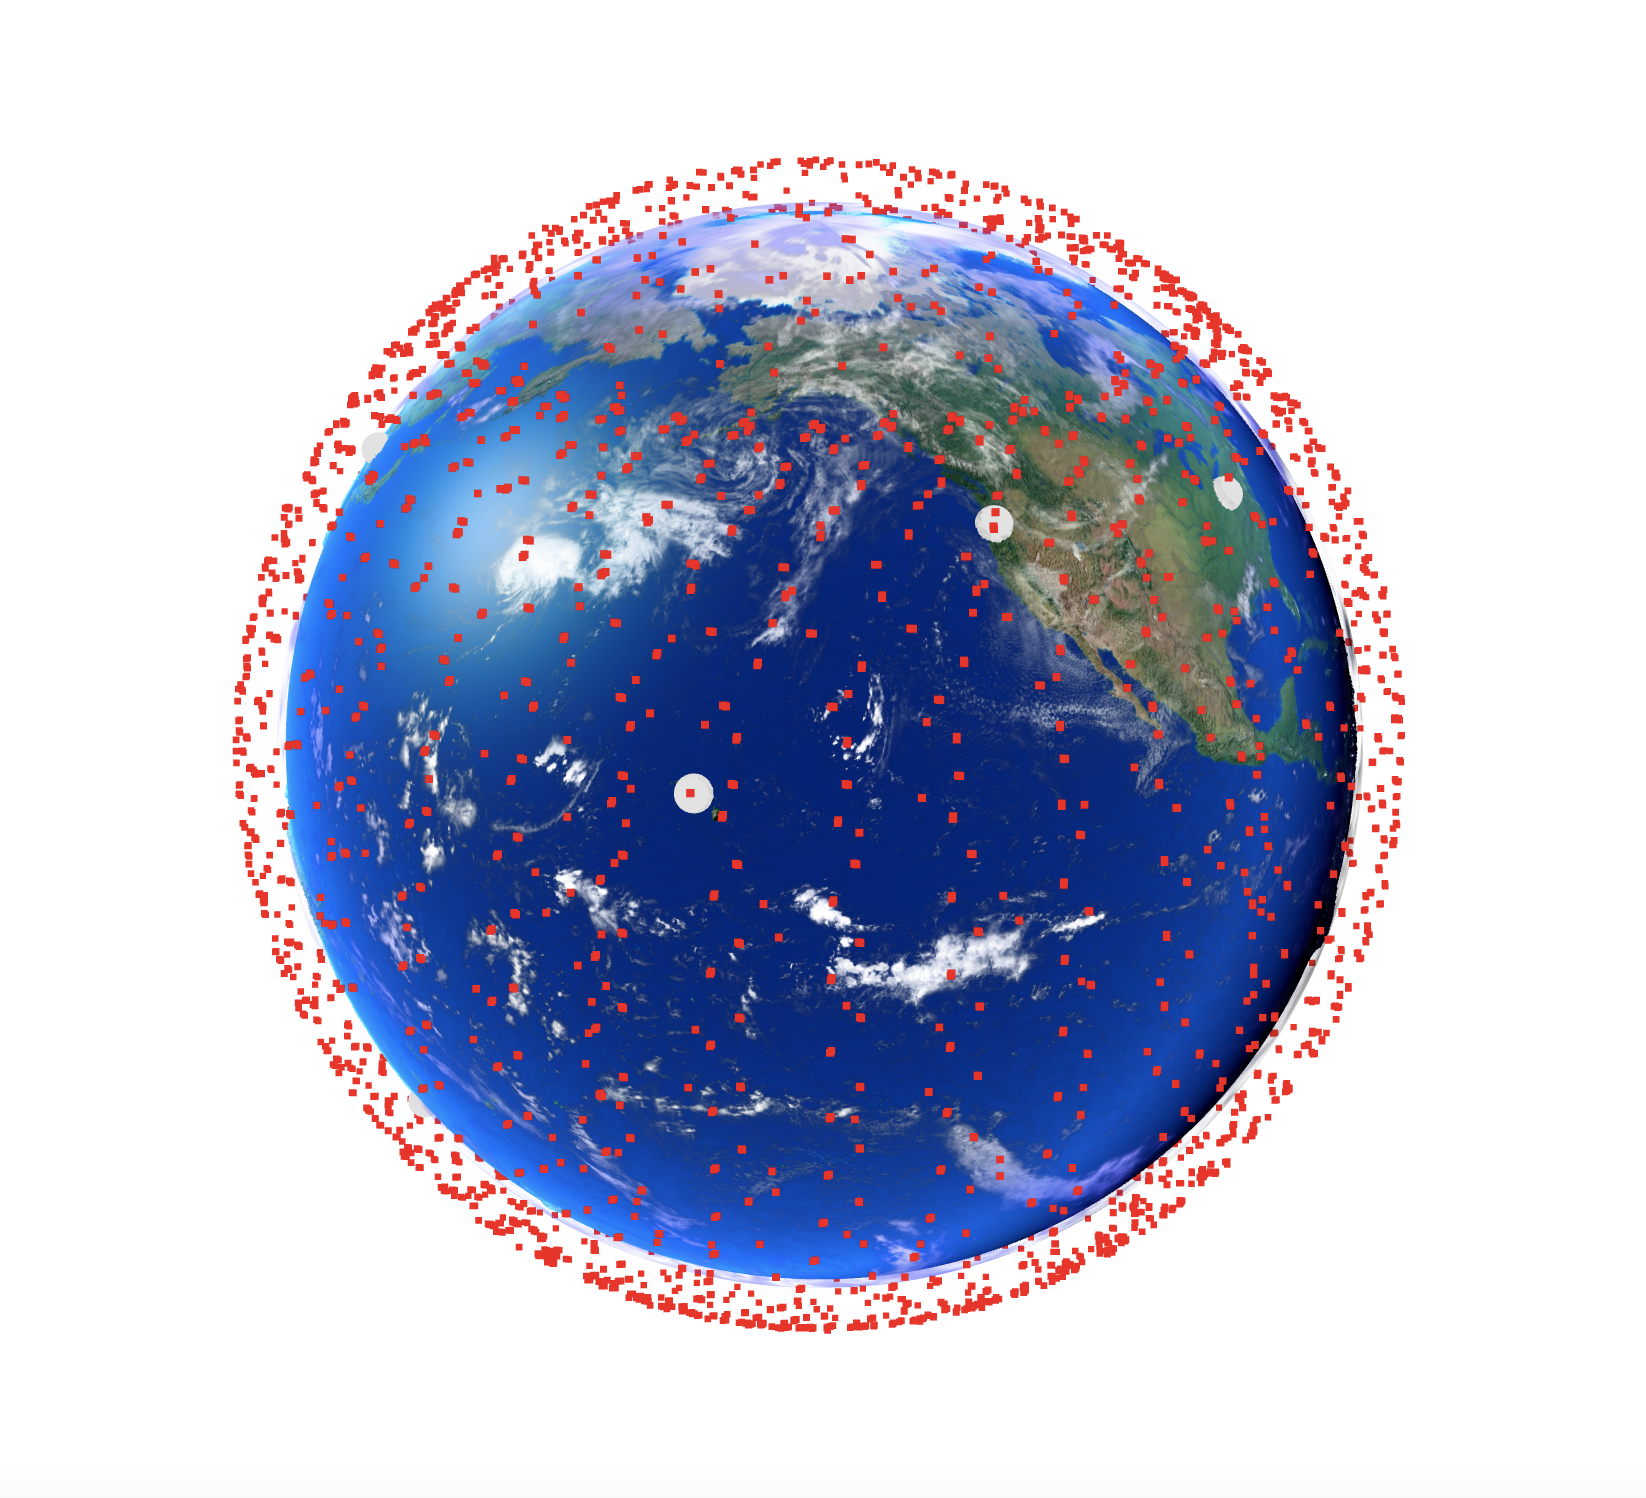
\includegraphics[width=\columnwidth]{images/starlinkphase1.png}
      \newline
      Starlink planned phase one deployment~\footnote[frame]{Image: Death by a Thousand COTS, Frederick Rawlins}
    \end{column}
  \end{columns}
\end{frame}

\begin{frame}
  \frametitle{What's new in space?}
  \framesubtitle{Commercially competitive launch providers}
  \begin{columns}[t]
    \begin{column}{5cm}
      \centering
      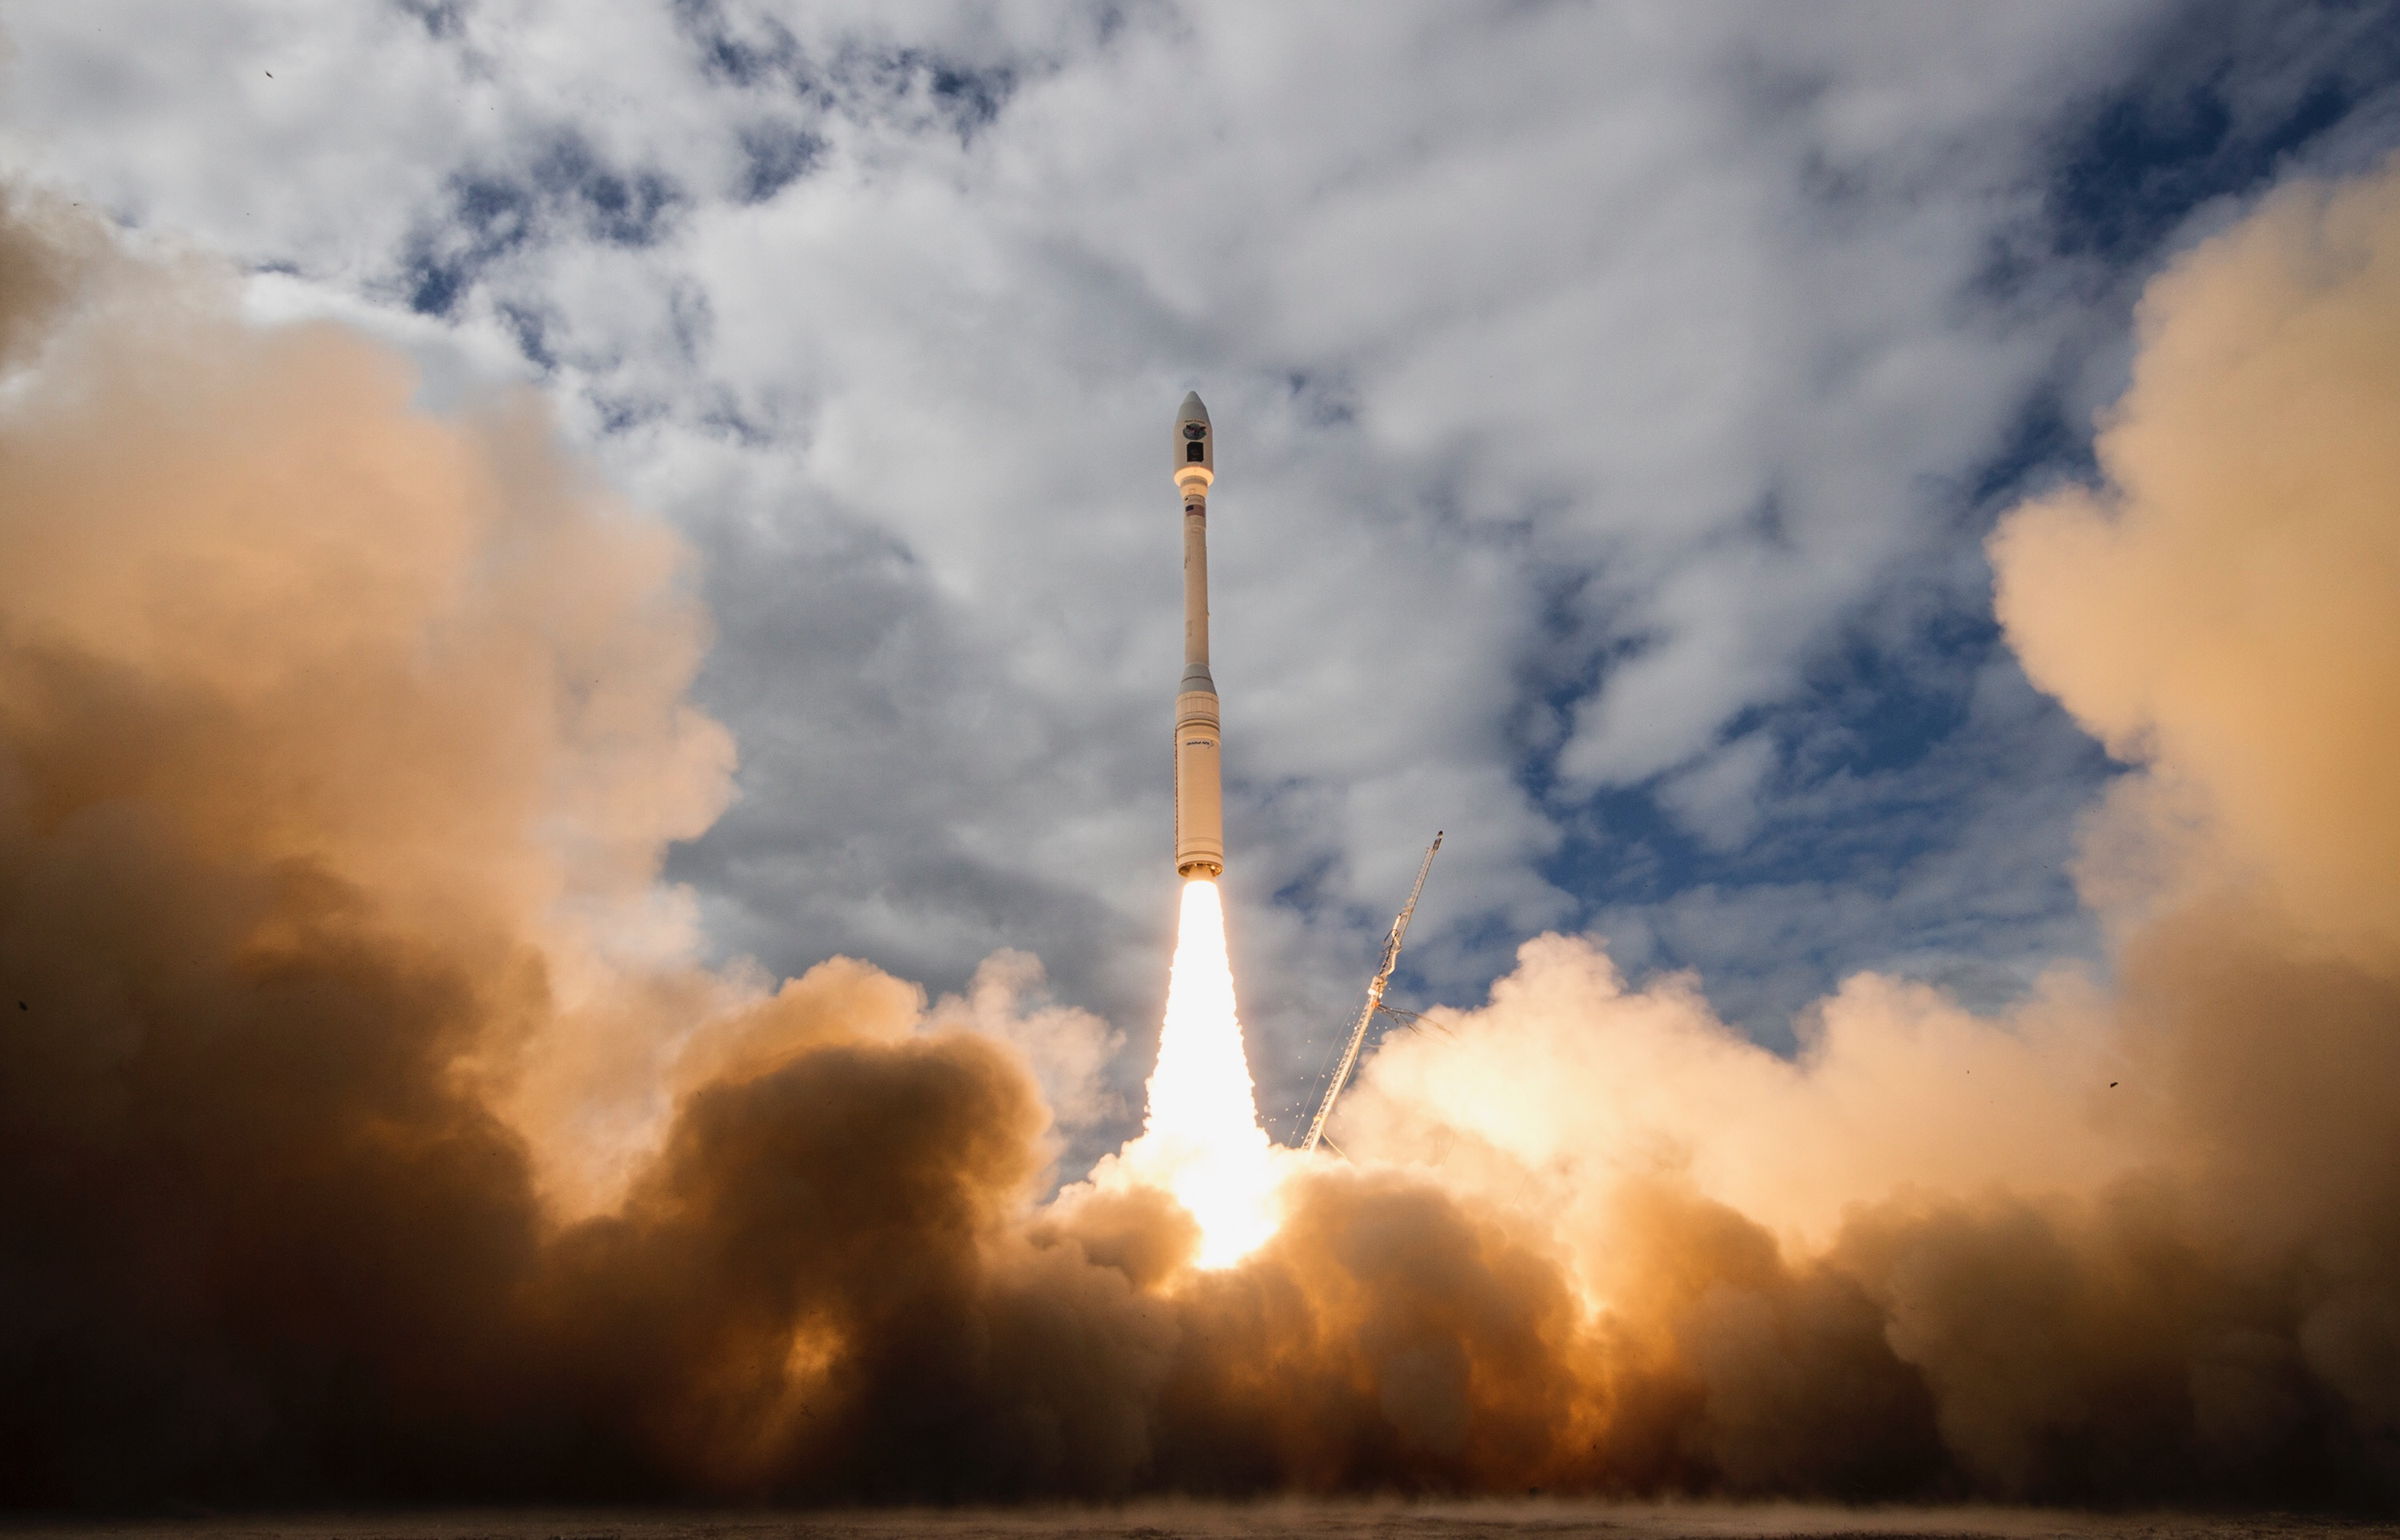
\includegraphics[width=0.8\textwidth]{images/planetlabs_launch.jpg}
      \newline
      Launch of SkySats 8-13 and Flock 3m~\footnote[frame]{Image: Orbital ATK}
    \end{column}

    \begin{column}{5cm}
      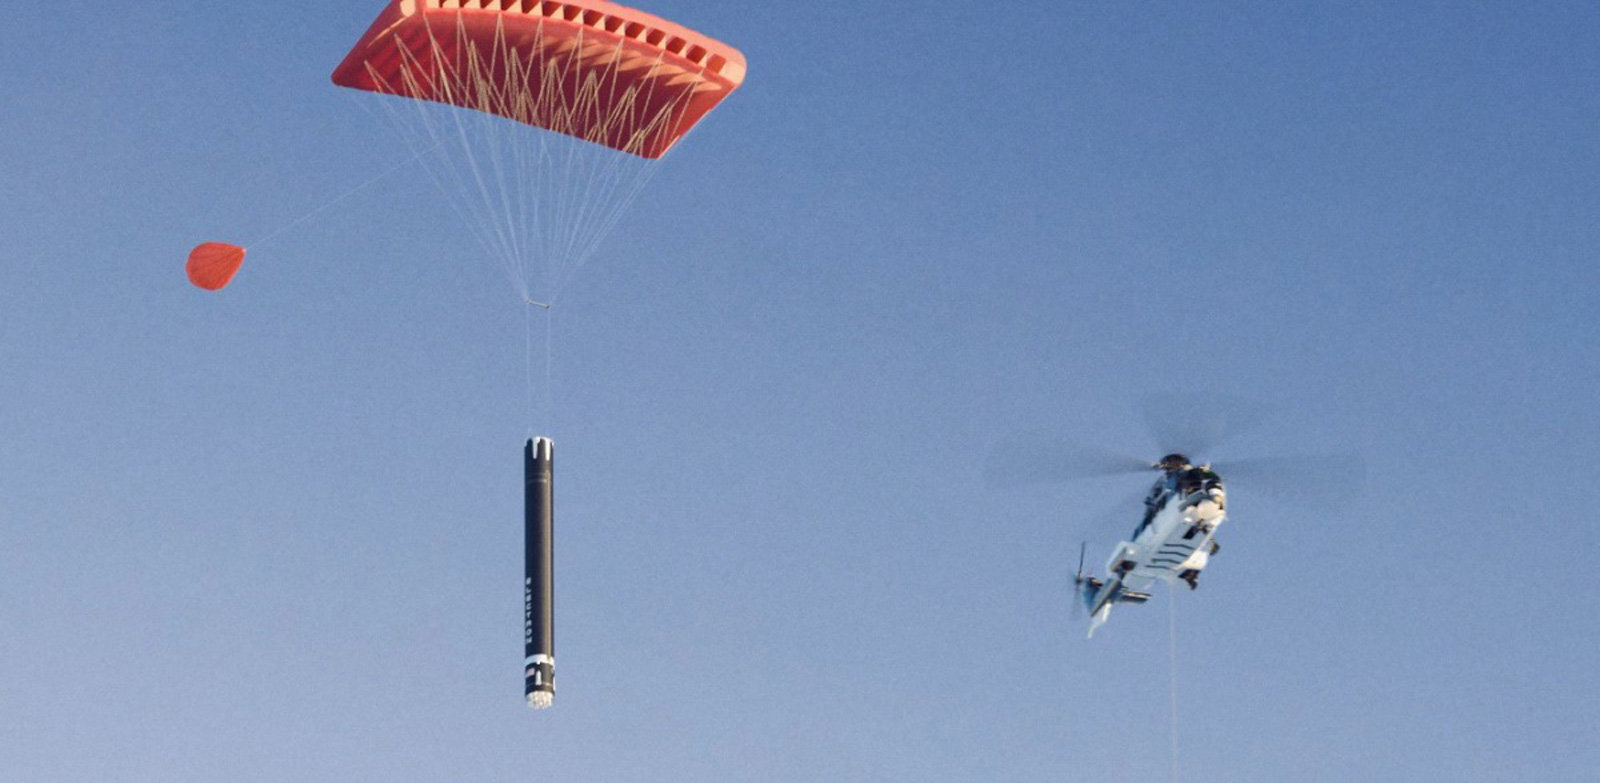
\includegraphics[width=0.8\textwidth]{images/rocket_lab_capture.jpeg}
      \newline
      In-air helicopter Rocket Labs capture~\footnote[frame]{Image: Rocket Labs}
    \end{column}

  \end{columns}
\end{frame}

\note{
  It's a really interesting time to research space systems, partially because with the dawn of so-called "new space", we're seeing unprecedented growth in the sector.
  Commercially competitive services are being developed to complement existing national space agencies to tackle problems such as Earth monitoring and global communications.

  Lots of new satellites are being launched, which are for the first time considering security throughout the entire design process.
  This has lead to the development of standardised protocols, encryption standards, and hardware.
}

\begin{frame}
  \frametitle{Reliance on old space}
  \begin{itemize}[<+->]
    \item Many legacy satellite systems currently exist
      \note<1>{
        However, while the security community is mostly focussed on making this new technology more secure, legacy satellite systems still exist.
      }
    \item They are widely used for research and national infrastructure
      \note<2>{
        Although these satellites were launched decades ago, many have outlived their planned lifespans to this day, and are still widely used for critical purposes such as forest fire detection and analysis of activities in conflict areas.

        However, the groundstations for these satellites are often receiving data which isn't securely authenticated.
        Instead, they implicitly trust that the input radio data is secure.
      }
    \item Since their launch, hardware and attack techniques have advanced
      \note<3>{
        When these satellites were launched, intercepting communications and performing injection attacks would have required infeasibly expensive and specialised hardware.  
        When combined with computational constraints on the satellites, it therefore sometimes made sense to transmit data in the clear.
        However, it is now commonly understood that commercially available hardware, such as the software defined radio, is sufficient to emit an attacking interference pattern in the vicinity of the receiver, resulting in data injection.
      }
    \item These satellites are vulnerable to new attack techniques
      \note<4>{
        Additionally, in the last few decades, our understanding of cryptography has advanced, with certain satellites using encryption algorithms that are now considered weak.
        This opens up previously secure satellites systems to the same kinds of signal injection attack.
        We expect more such systems to be affected as cryptography advances and quantum computing breaks previously secure algorithms.
    It is now well accepted that legacy computing systems which trust their input data aren't resilient against modern adversaries.
    However, no current research exists to determine which satellites are affected, how difficult it is to pull off such an attack, or what the ramifications would be.
      }
  \end{itemize}
\end{frame}

% Since the advent of the software-defined radio, mounting an injection attack against an insecure satellite downlink requires only access to off-the-shelf hardware
% There's no current research investigating the impact of a modern adversary overshadowing Earth monitoring satellites

\section{Background}
\subsection{Satellite downlink communications}
% TODO: simplify diagram
\begin{frame}
  \frametitle{Satellite downlink communications}
  \centering
  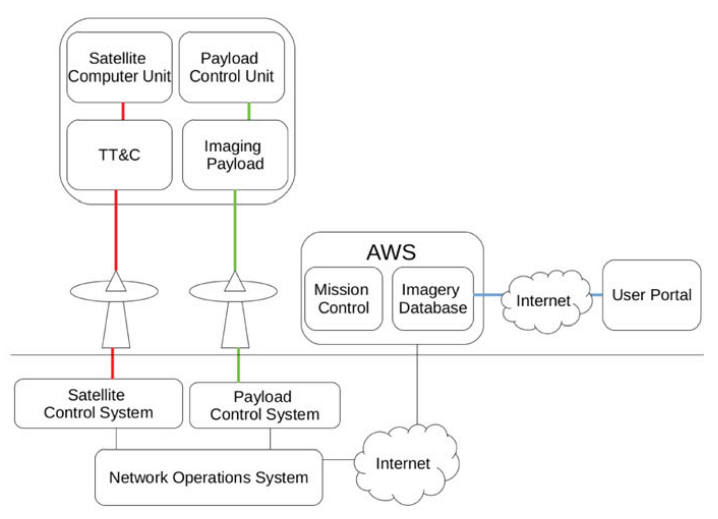
\includegraphics[width=0.65\textwidth]{images/dataset_generation.png}
  \newline
  \textit{Ground segment architecture for web-based access}
  \newline

  \onslide<2>
  If an attacker can control the communications, they can affect the derived datasets.

  \note{
    From satellite, through some processing system, and then out via the internet
    Now of course, if a satellite implements good cryptographic authenticity, then an attacker can only deny service through jamming the physical layer. However against an unencrypted satellite downlink, the attacker can potentially affect the communications in much more subtle ways.
  }
\end{frame}

% TODO: split previous notes across to this slide

\subsection{Threat model}
\begin{frame}
  \frametitle{Threat model}
  \framesubtitle{Adversary's goal}
  Cause disruption to downlink processing systems by emitting counterfeit signals in the vicinity of the receiver, resulting in either:
  \newline

  \begin{itemize}
    \item Affecting the satellite-derived datasets:
    \begin{itemize}
      \item Inject false data, disrupting automated detection systems.
      \item Mask real data, denying people information.
    \end{itemize}
    \item Exploiting or disrupting downlink processing stages:
    \begin{itemize}
      \item Achieve denial of service, e.g. by causing pipeline stages to crash.
      \item Execute arbitrary code, e.g. by exploiting processing stages that call the shell.
    \end{itemize}
  \end{itemize}
\end{frame}

\section{Contributions}

\begin{frame}
  \frametitle{Contributions}
  \begin{itemize}
    \item Understand the effect that a modern adversary can have against legacy satellite downlinks.
    \item End-to-end case study on real world forest fire detection systems.
    \item Evaluate the impact of the attack, in
      \begin{itemize}
        \item poisoning the dataset.
        \item exploiting the processing software.
      \end{itemize}
    \item Examine the feasibility of performing the attack in the real world.
    \item Understand the available countermeasures.
  \end{itemize}

  \note{
    In this talk, we'll be discussing what happens when a modern adversary exploits the implicit trust of legacy groundstations.
    In particular, we'll consider the effects of an attacker injecting data by emitting a counterfeit radio signal in the vicinity of a receiver.

    We'll illustrate the problem through an end-to-end case study on FIRMS, which is NASA's real time forest fire detection system.
    This system provides a live map of all significant forest fires on Earth, and it's used in over 160 countries including by national firefighting services.

    We demonstrate that, by controlling the input data, an attacker can mislead crisis response by two different means:
    Firstly, they can poison the output dataset.
    This means either injecting their own ficticious forest fires, or masking existing ones.
    Secondly, they can exploit the processing systems themselves.
    Since NASA's receiver software implicitly trusts the input data to be of the correct format, we show how an attacker can violate these assumptions to crash the system or achieve arbitrary code execution.

    We go on to examine the feasibility of performing the attack in the real world.
    This means investigating the budgetary constraints of an attacker, as well as considering the physical radio things they'll have to overcome.

    Finally, we
 }
  
  \note{In this talk, we'll consider the effect of a modern adversary against NASA's live forest fire detection system, as used in over 160 countries.
  We'll demonstrate end-to-end how overshadowing the physical layer can lead to poisoning the satellite-derived datasets and exploiting the processing systems themselves.
  We demonstrate that an attacker can arbitrarily manipulate fires in the derived dataset to trigger false emergency response or mislead crisis analysis.
  Finally, we demonstrate through radio simulation that it's practical for a ground-based attacker to achieve the required signal injection attack, even against a highly directional dish.
  }
\end{frame}

\section{Attack}
\subsection{Forest fire detection}
\begin{frame}
  \frametitle{Forest fire detection}
  \framesubtitle{FIRMS: NASA's global fire detection service}
  \centering
  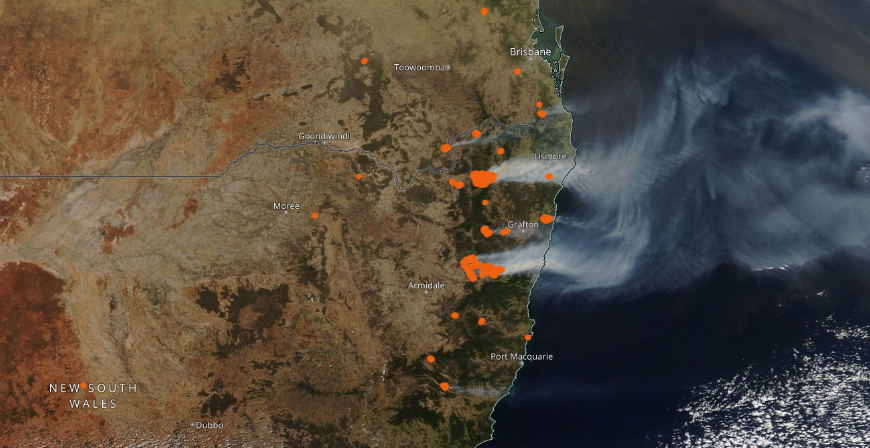
\includegraphics[width=\columnwidth]{images/bushfire.png}
  \newline
  The 2019 Australia bushfires as seen from Aqua's MODIS instrument, annotated with the \textit{Fires and Thermal Anomalies} dataset on NASA's worldview.
\end{frame}

\subsection{Attack overview}

\begin{frame}
  \frametitle{Attack overview}
  \framesubtitle{Overshadowing the physical layer}
  \centering
  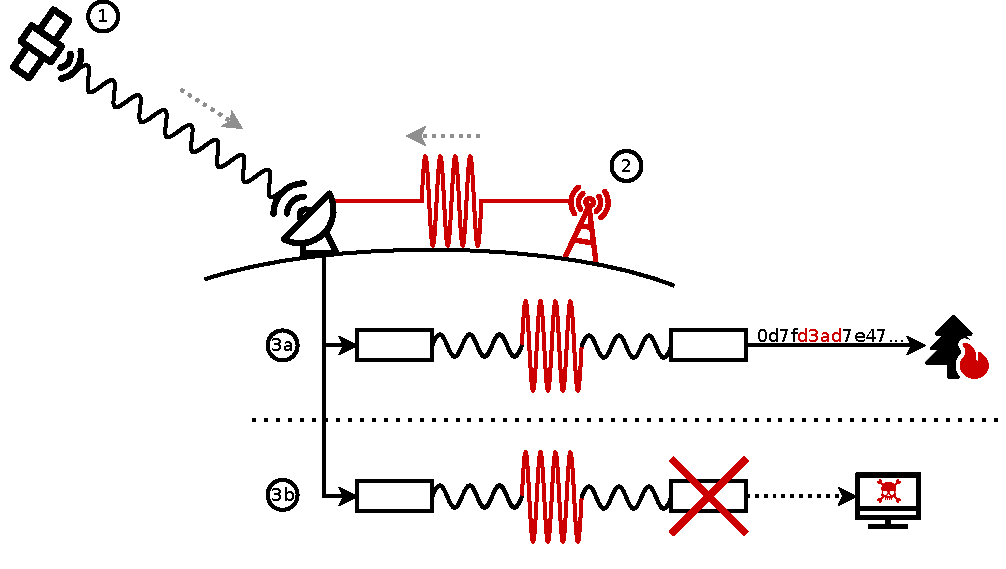
\includegraphics[width=0.7\textwidth]{images/attack_illustration.pdf}
  \begin{enumerate}
    \item The satellite broadcasts a signal.
    \item Attacker injects a crafted signal.
    \item The attacker-controlled data decodes, resulting in either:
      \begin{enumerate}
        \item[a)] affecting the derived datasets.
        \item[b)] exploiting the processing stages.
      \end{enumerate}
  \end{enumerate}
\end{frame}

% \begin{frame}
%   % Attack data generation
%   \frametitle{Attack overview}
%   \begin{itemize}
%     \item Construct attack data packets, by either;
%       \begin{itemize}
%         \item Tampering with image data to affect derived datasets.
%         \item Violating the packet protocols, to exploit processing stages.
%       \end{itemize}
%     \item Reencode into raw samples;
%       \begin{itemize}
%         \item Implement a data link protocol encoder and generate the raw data frames.
%       \end{itemize}
%     \item Inject the radio signal;
%       \begin{itemize}
%         \item Modulate the data onto the correct frequency.
%         \item Amplify to overshadow the legitimate signal in the vicinity of the receiver.
%       \end{itemize}
%   \end{itemize}
% \end{frame}

\subsection{Affecting the derived datasets}

% TODO: expand into slides showing how
\begin{frame}
  \frametitle{Affecting the derived dataset}
  \framesubtitle{Overview}
  \begin{itemize}
    \item Obtain/capture legitimate data
    \begin{itemize}
      \item Beforehand -- download from NASA distributed data archive
      \item Live -- set up custom receiver setup
    \end{itemize}

    \item Process it to add/remove artefacts
    \begin{itemize}
      \item Reverse engineer the image format, and write an image manipulation program
    \end{itemize}
  \end{itemize}
\end{frame}

% \begin{frame}
%   \frametitle{Affecting the derived dataset}
%   \framesubtitle{Data capture}
%   \begin{itemize}
%     \item Derived datasets from Aqua available from distributed web archives from NASA's website
%     \item The files are separated according to a timestamp format, so the attacker needs to find an image of the desired location by using the satellite's orbital parameters
%   \end{itemize}
%   
%   \url{https://ladsweb.modaps.eosdis.nasa.gov}
% 
% \note{
%   LADSWeb archive - can download datasets at several different levels of processing
%   We want the lowest form possible
%   To know what to download, we need to do some reversing of the satellite coordinates and timestamp etc
%   Can theoretically do this in the live setting as well
% }
% \end{frame}

\begin{frame}
  \frametitle{Affecting the derived dataset}
  \framesubtitle{Data capture}
  \centering
  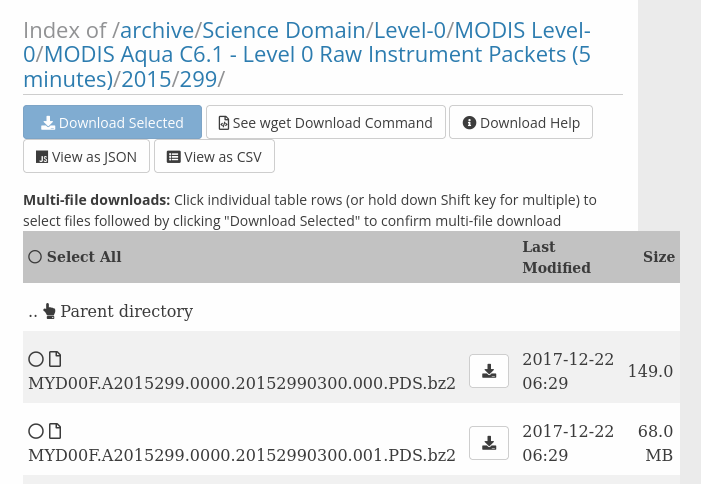
\includegraphics[width=0.8\textwidth]{images/level0.png}
  \url{https://ladsweb.modaps.eosdis.nasa.gov/archive/}
\end{frame}

\begin{frame}
  \frametitle{Affecting the derived dataset}
  \framesubtitle{Data processing: image format reversing}
  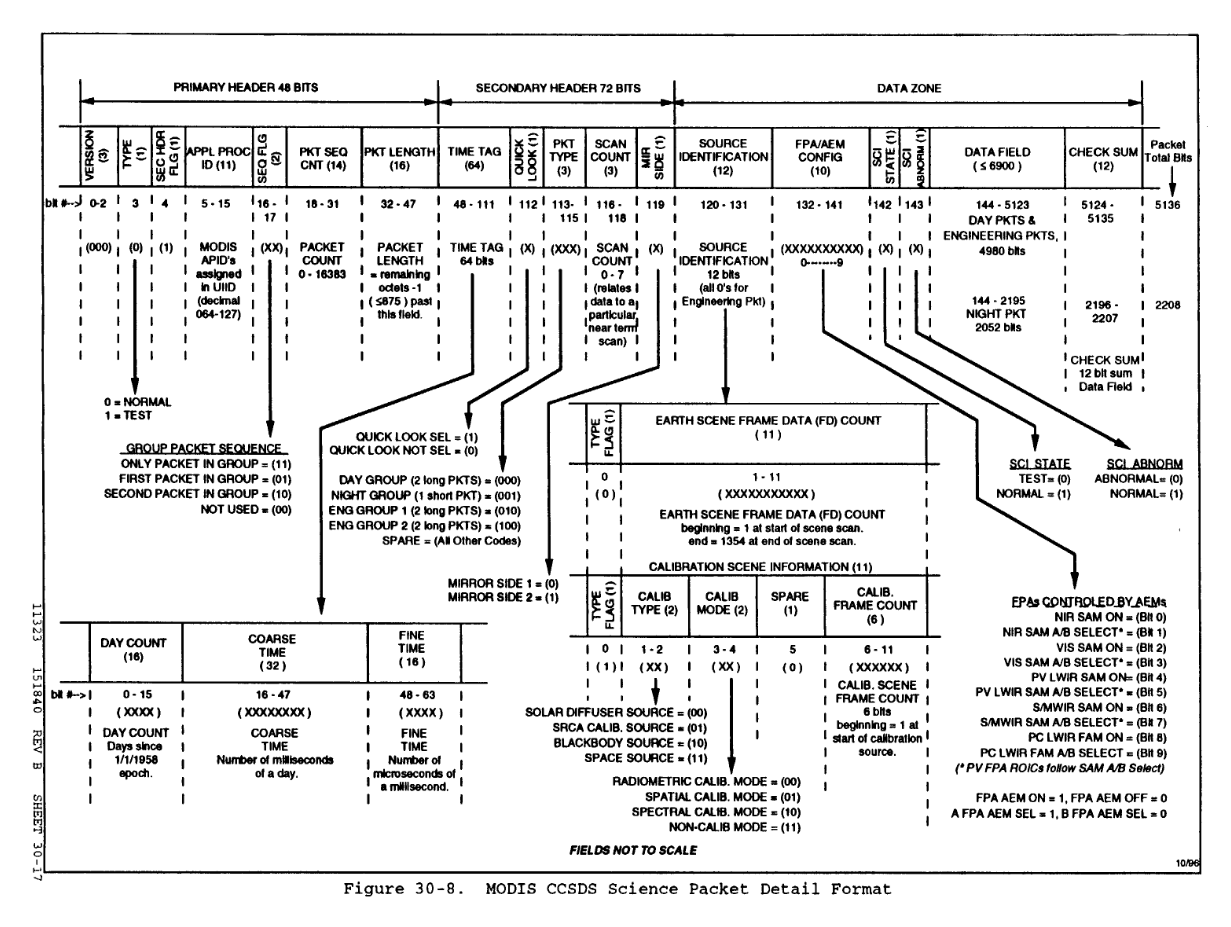
\includegraphics[width=\textwidth]{images/image_format.png}
\end{frame}

\subsection{Exploiting processing stages}

\begin{frame}
  \frametitle{Exploiting processing stages}
  \framesubtitle{Overview}
  \begin{itemize}
   \item Obtain downlink decoder software and perform security audit
   \begin{itemize}
     \item Look for possible exploits around manual memory management and execution boundaries
   \end{itemize}
    \item Construct payload packet to trigger vulnerability chain
    \begin{itemize}
      \item Violate assumptions about the protocol headers
    \end{itemize}
  \end{itemize}
\end{frame}

\begin{frame}
  \frametitle{Exploiting processing stages}
  \framesubtitle{Obtaining the processing software}
  \centering
  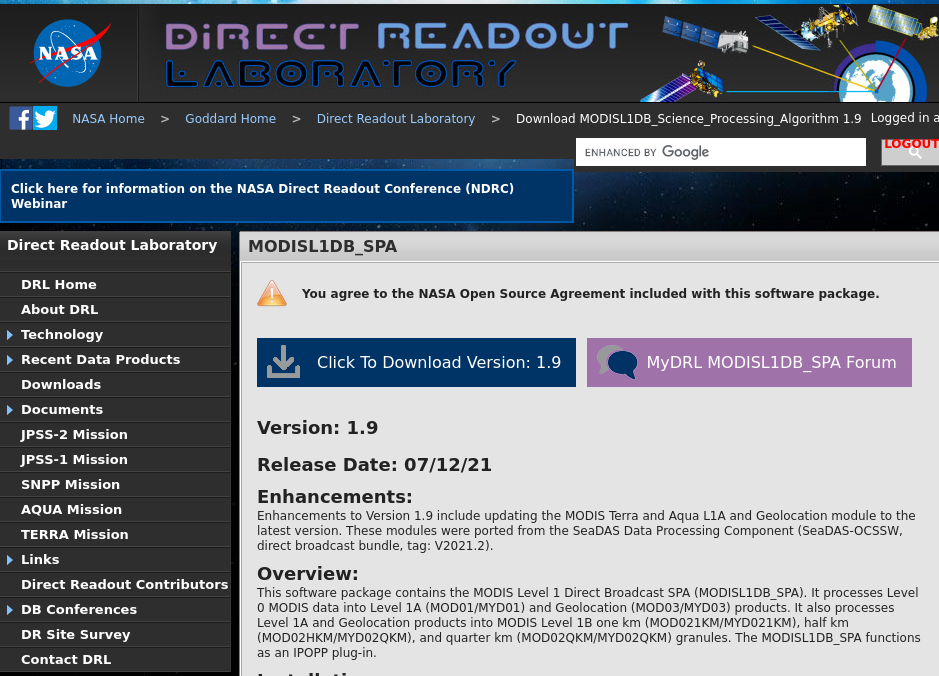
\includegraphics[width=0.7\textwidth]{images/drl.png}
  \newline
  With a research account, anyone can download the entire set of decoding software from NASA's \textit{Direct Readout Laboratory}
  \newline
  \url{https://directreadout.sci.gsfc.nasa.gov/}
\end{frame}

\begin{frame}
  \frametitle{Exploiting processing stages}
  \framesubtitle{Construct payload packet}
  \centering
  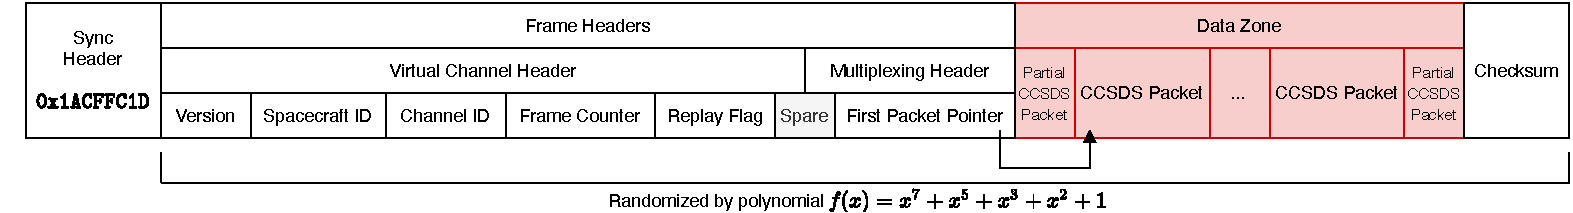
\includegraphics[width=\textwidth]{images/cadu_diagram.pdf}
  \note{Number of causes of concern: L0 to L1 made of many disparate components, interacting across boundaries with access to the shell. Using C programs that don't pay huge attention to managing memory correctly, and using a slightly buggy protocol header parser.}
\end{frame}

\section{Evaluation}
\subsection{Experimental setup}

\begin{frame}
  \frametitle{Experimental setup}
  \framesubtitle{End-to-end evaluation pipeline}
  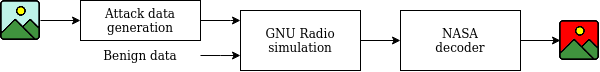
\includegraphics[width=\textwidth]{images/overall_simulation.png}
\end{frame}

\begin{frame}
  \frametitle{Experimental setup}
  \framesubtitle{GNU Radio simulation}
  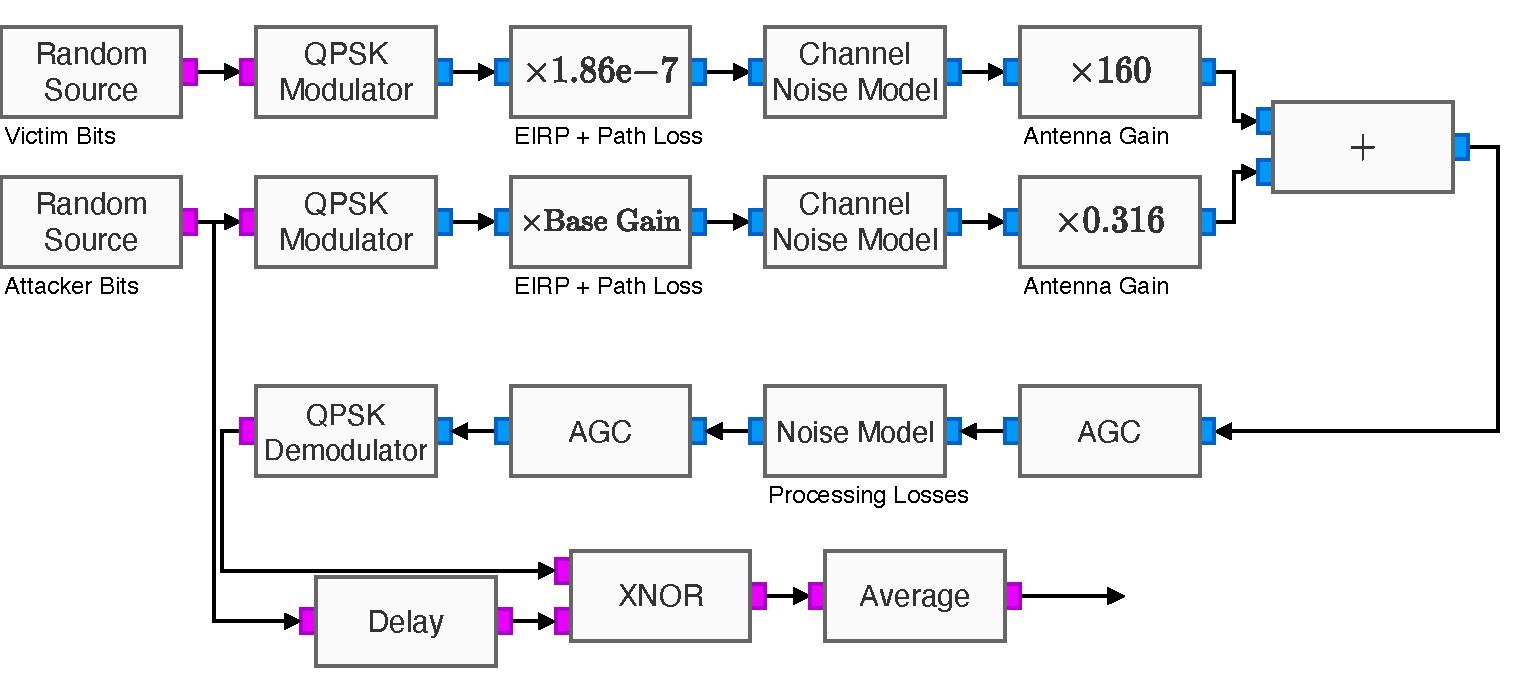
\includegraphics[width=\textwidth]{images/overshadowing_pipeline.pdf}
\end{frame}

\begin{frame}
  \frametitle{Experimental setup}
  \framesubtitle{NASA decoder}
  \centering
  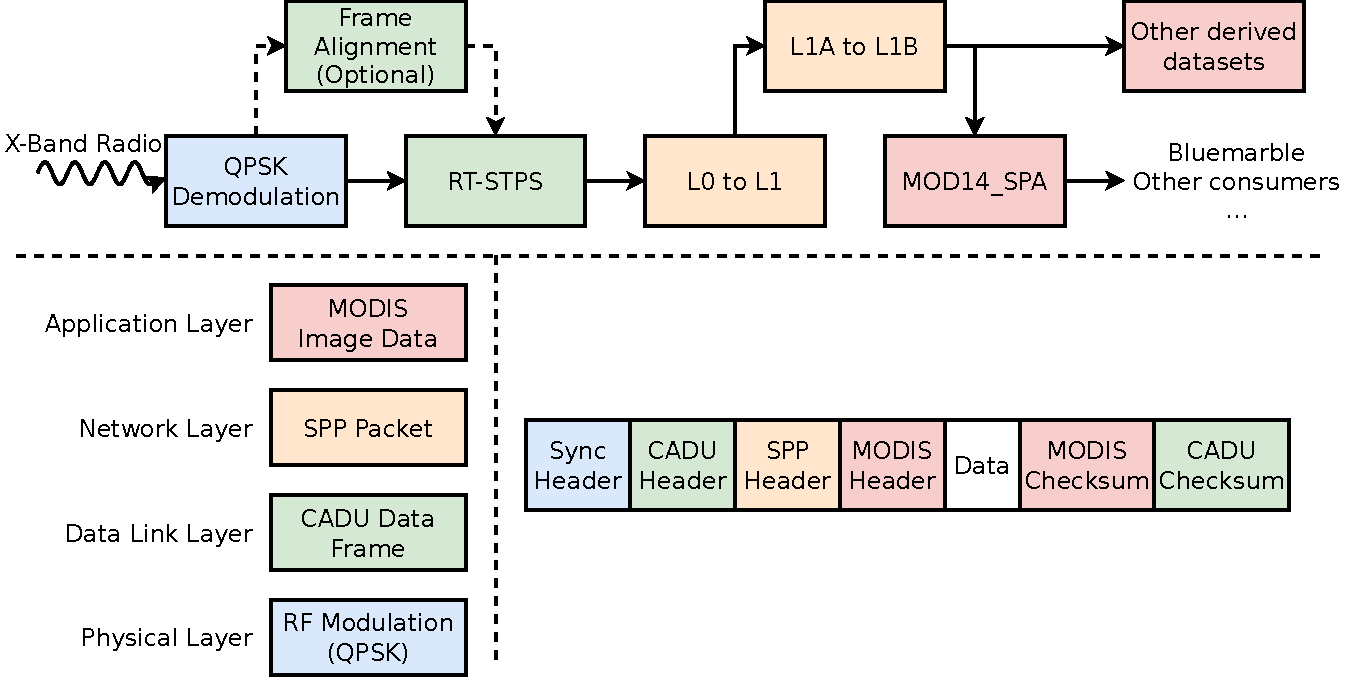
\includegraphics[width=0.8\textwidth]{images/attack_types.pdf}
  \url{https://github.com/ssloxford/firefly/tree/master/decoder_pipeline}
\end{frame}

\subsection{Attack consequences}

% TODO: tie into how this misleads crisis response
\begin{frame}
  \frametitle{Attack consequences}
  \framesubtitle{Affecting the derived dataset}
  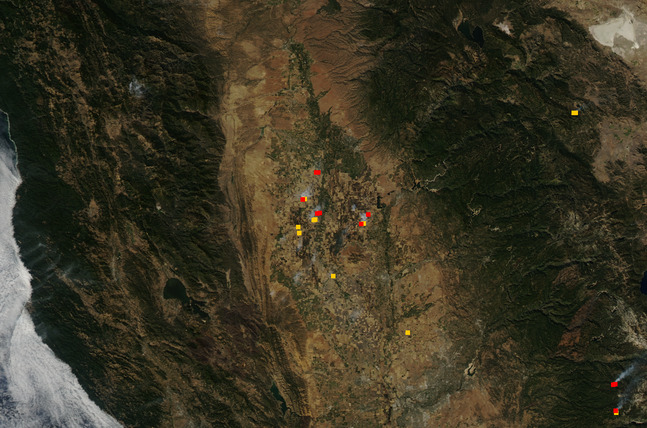
\includegraphics[width=\textwidth]{images/injection/original.jpg}
  \newline
  \centering
  Original image.
\end{frame}

\begin{frame}
  \frametitle{Attack consequences}
  \framesubtitle{Affecting the derived dataset}
  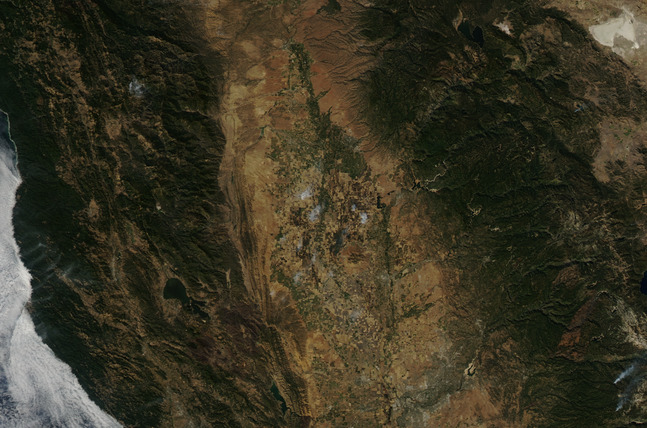
\includegraphics[width=\textwidth]{images/injection/masked_0.jpg}
  \newline
  \centering
  Masking existing fires.
\end{frame}

\begin{frame}
  \frametitle{Attack consequences}
  \framesubtitle{Affecting the derived dataset}
  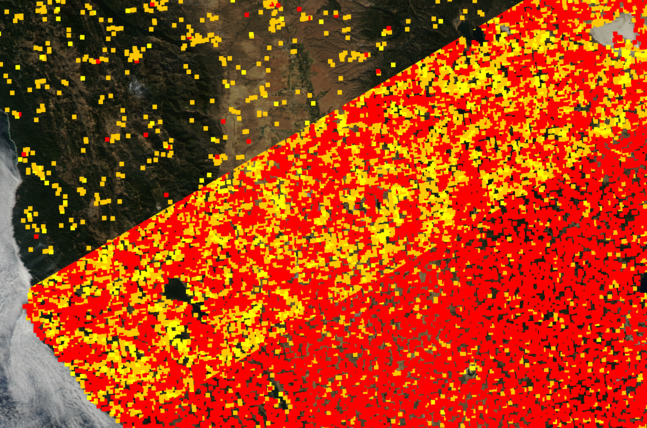
\includegraphics[width=\textwidth]{images/injection/random_combined_diagonal.jpg}
  \newline
  \centering
  Injecting uniform ficticious fires.
\end{frame}

\begin{frame}
  \frametitle{Attack consequences}
  \framesubtitle{Affecting the derived dataset}
  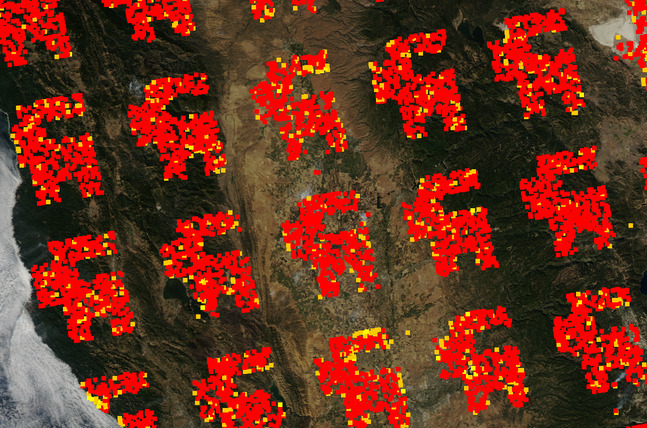
\includegraphics[width=\textwidth]{images/injection/amogi.jpg}
  \newline
  \centering
  Injecting ficticious fires with fine-grained control.
\end{frame}

\begin{frame}
  \frametitle{Attack consequences}
  \framesubtitle{Exploiting the processing stages}
  \centering
  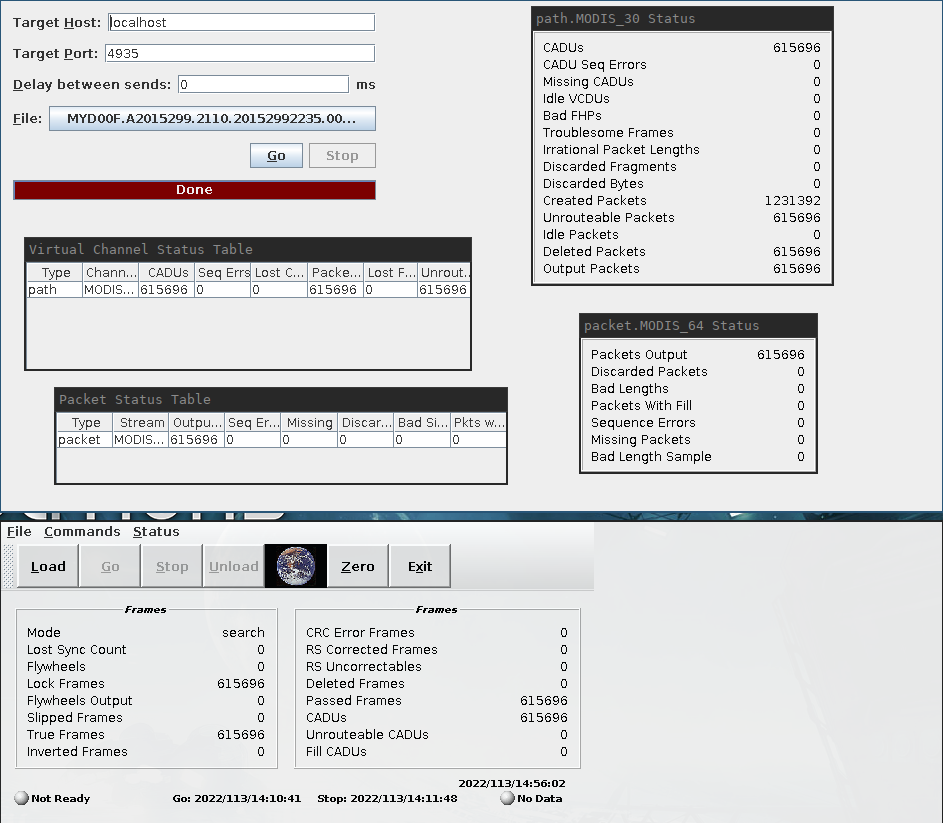
\includegraphics[width=0.7\textwidth]{images/rtstps_correct.png}
\end{frame}

\begin{frame}
  \frametitle{Attack consequences}
  \framesubtitle{Exploiting the processing stages}
  \centering
  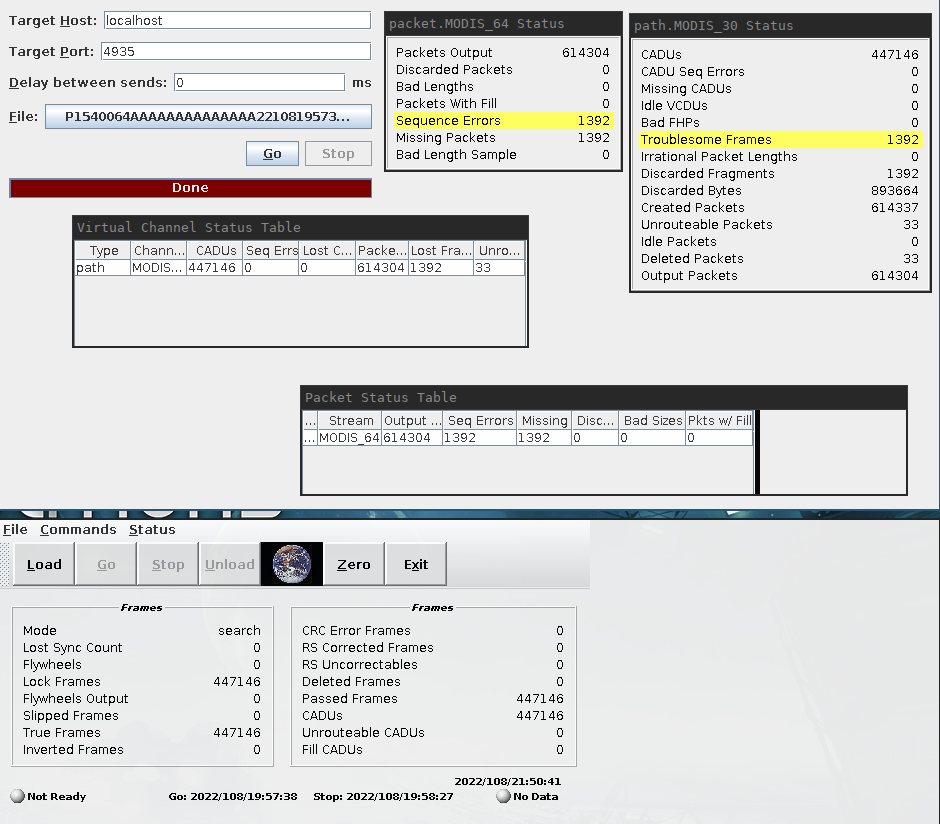
\includegraphics[width=0.7\textwidth]{images/rtstps_incorrect.png}
\end{frame}


\subsection{Attacker capabilities}

\begin{frame}
  \frametitle{Attacker capabilities}
  \framesubtitle{Estimated cost}
  \centering
  \begin{tabular}{ l | l }
    \textbf{Hardware component} & \textbf{Cost} \\
    \hline
    limeSDR & $598$ USD \\
    X-Band transmitter & $22,800$ EUR \\
    Compatible antenna & $6,400$ EUR \\
    \hline
    Total & \~{}$30,000$ EUR
  \end{tabular}

  Within the budget of a motivated hobbyist.
\end{frame}

\begin{frame}
  \frametitle{Attacker capabilities}
  \framesubtitle{Results}
  \begin{figure}
      \centering
      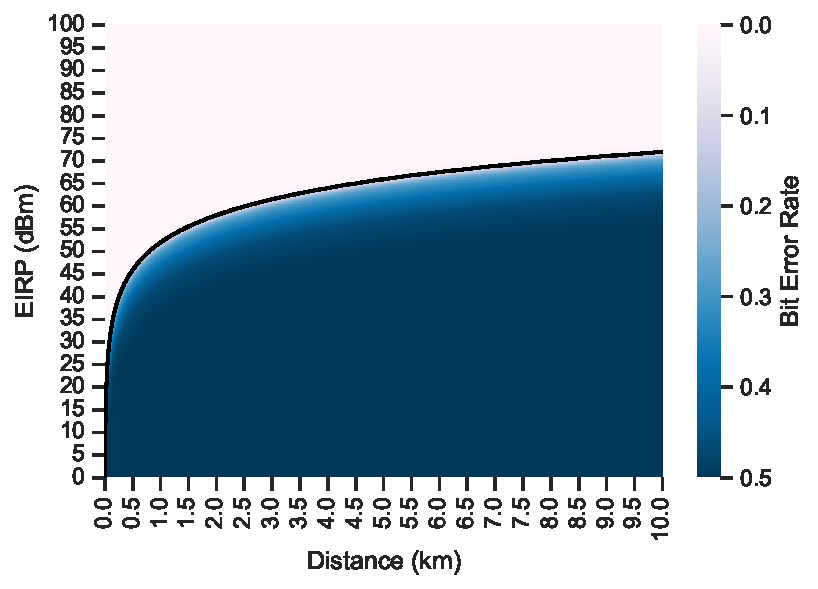
\includegraphics[width=0.6\columnwidth]{images/distance_eirp_heatmap_95.pdf}
      \caption{The bit error rate of the injected signal as the attacker varies EIRP and distance from the receiver. The values beyond which the bit error rate drops below $5$\% are indicated using a line.}
      \label{fig:distance_eirp}
  \end{figure}
  Our transmitter has EIRP (Effective Isotropic Radiated Power) of 49dBm.
\end{frame}

\section{Discussion}

\subsection{Countermeasures}

\begin{frame}
  \frametitle{Countermeasures}
  \framesubtitle{Cryptographic solutions}
  \begin{itemize}
    \item Cryptographic solutions
    \item Timing analysis
    \item Waveform analysis
    \item Data inspection
  \end{itemize}

  \note{
    Crypto:
    Gives strong guarantees of data integrity, authenticity, non-repudiation, etc.
    Satellites have long lifespans, so currently secure crypto might become breakable (post-quantum)
    Retrofitting crypto onto existing satellite systems is infeasible

    Timing:
    Multiple receiver triangulation to determine attacker location
    Requires coordination between multiple groundstations

    Waveform:
    Looking at properties of the legitimate/overshadowed signal
    Traditional approaches like analysing signal-to-noise may prove effective
    New ML approaches starting to be created (PAST-AI)

    Data:
    Look for artefacts of tampering in the packets, and compare packets from multiple groundstations
    Doesn't require any hardware modifications to the receiver
    Protects against decoder exploitation
    Doesn't protect against dataset poisoning
  }
\end{frame}

\subsection{Generalisability}

\begin{frame}
  \frametitle{Generalisability}
  \framesubtitle{Other vulnerable satellites}
  \begin{columns}[t]
    \begin{column}{4cm}
      \begin{figure}
          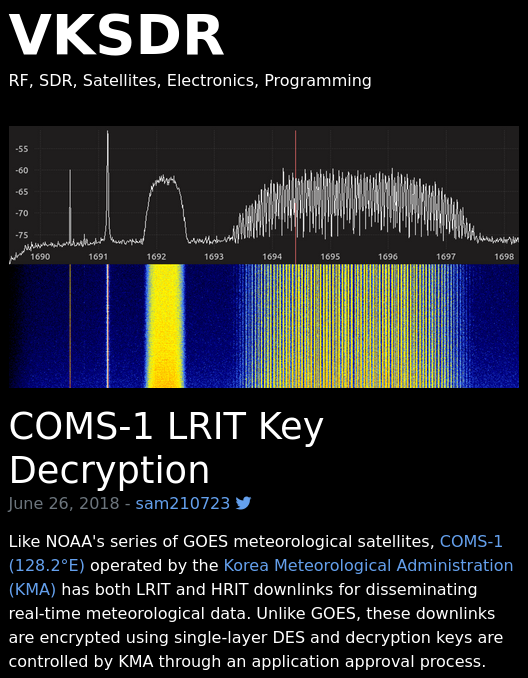
\includegraphics[width=\columnwidth]{images/lrit-key-dec.png}
          \label{fig:lrit-key-dec}
      \end{figure}
    \end{column}

    \begin{column}{4cm}
      \begin{figure}
          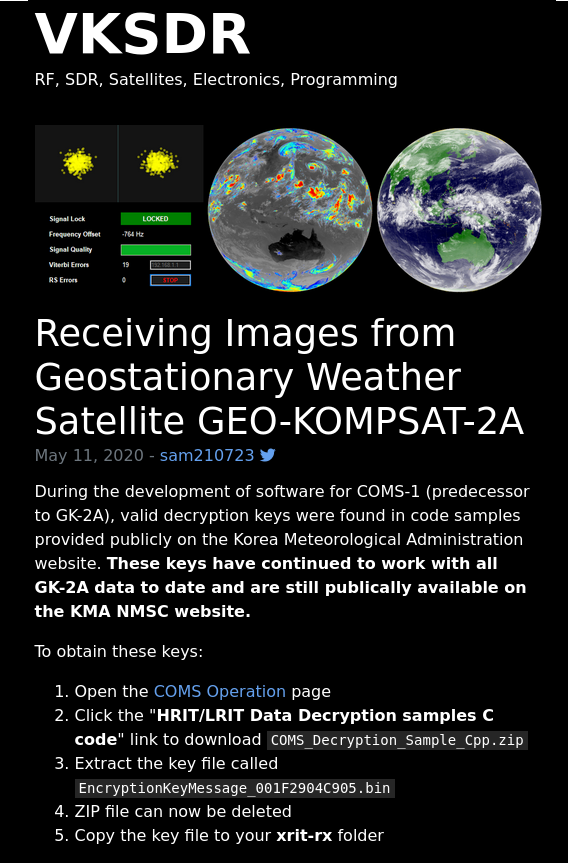
\includegraphics[width=\columnwidth]{images/xrit-rx.png}
          \label{fig:xrit-rx}
      \end{figure}
    \end{column}

  \end{columns}
  \url{https://vksdr.com/}
  \note{
    Mention post-quantum
    Explain how a combination of weak crypto (DES 1), hardcoded keys, and and bad key management has lead to these Korean satellites being essentially unencrypted
    It's hard to blame anyone - the threat landscape has shifted so much
    crypto has come along a long way, and these satellites are up for decades or more
  }
\end{frame}

\begin{frame}
  \frametitle{Generalisability}
  \framesubtitle{Other vulnerable systems}
  Using Terra/Aqua data:
  \begin{itemize}
    \item \url{https://www.cloudtostreet.ai/}
      \begin{itemize}
        \item Flood tracking (disasters and insurance)
      \end{itemize}
    \item \url{https://ncx.com/basemap/}
      \begin{itemize}
        \item Timber and carbon value monitoring in the USA
      \end{itemize}
    \item \url{https://www.upstream.tech/hydroforecast}
      \begin{itemize}
        \item Water flow and weather intelligence
      \end{itemize}
  \end{itemize}

  \onslide<2>
  Using other potentially vulnerable systems:
  \begin{itemize}
    \item \url{https://maps.google.com}
      \begin{itemize}
        \item Uses data from the GOES fleet, which is known decryptable
      \end{itemize}
    \item Services derived from LandSat
      \begin{itemize}
        \item Deforestation
        \item Water conservation
        \item Was subject to attacking interference, going unnoticed for a year
      \end{itemize}
  \end{itemize}

  \onslide<2>
  % Code
\end{frame}

\begin{frame}
  \frametitle{Generalisability}
  \framesubtitle{Reproducing the work}
  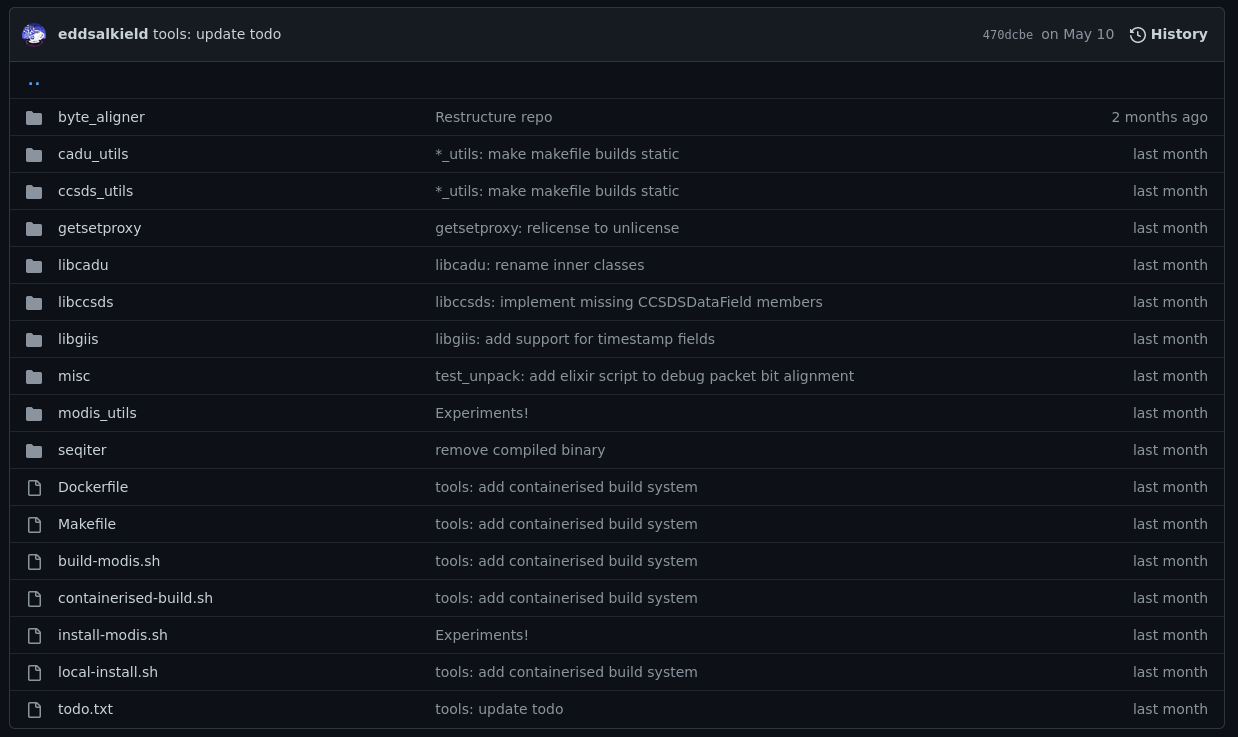
\includegraphics[width=\textwidth]{images/code_overview.png}
\end{frame}

\begin{frame}
  \frametitle{Generalisability}
  \framesubtitle{Reproducing the work}
  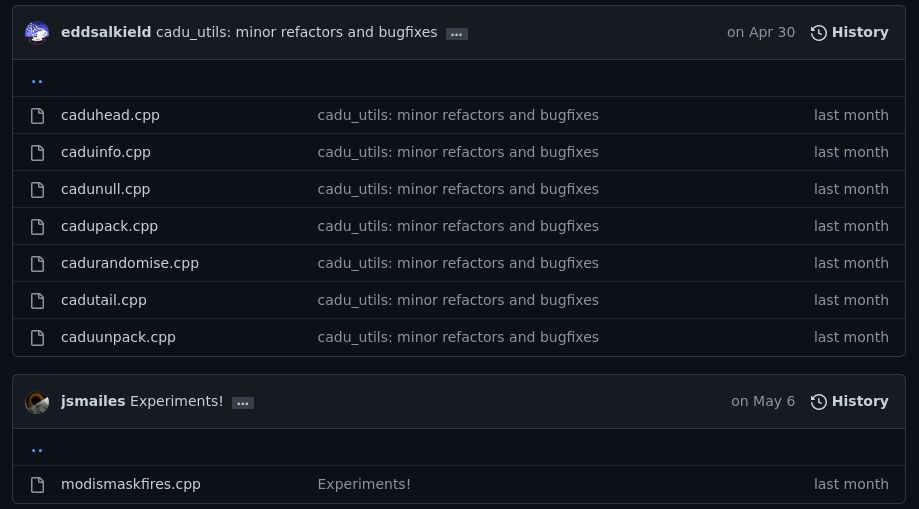
\includegraphics[width=\textwidth]{images/code_tools.png}
\end{frame}

\section{Conclusion}

\begin{frame}
  \frametitle{Conclusion}
  \begin{itemize}
    \item Signal injection against satellite downlinks are currently effective against decryptable classes of satellites
    \item Through an end-to-end case study, we demonstrated that NASA's fire detection system is vulnerable, with wide ramifications
    \item Only a moderate equipment budget is required to perform these attacks
    \item Currently proposed countermeasures would increase the complexity of performing this attack in practice
    \item Future work should consider a comprehensive overview of similarly vulnerable systems
  \end{itemize}
\end{frame}

% TODO: end card with socials, contact details, etc.

\end{document}
